\chapter{Introduction}
\label{chap:introduction}

The proliferation of cloud storage, content distribution networks, and 
public curated datasets poses new challenges and
opportunities for hosting data.  On the one hand, the availability of
professionally-maintained services is a boon to developers, since it lets them
offload the operational burden of hosting data.  On the other
hand, it is difficult to leverage these services over long
timescales.  Services can appear and disappear, and service operators can
unilaterally change their APIs, pricing, and trustworthiness.
Over long enough timescales, developers find themselves continuously
patching their applications to accommodate new service behaviors.

This thesis presents a novel storage architecture, called \emph{wide-area
software-defined storage} (SDS), that helps developers
leverage these commodity services without this constant patching.
In SDS, developers specify their desired
\emph{end-to-end storage semantics} independently of
both applications and underlying services.  The storage semantics define the
rules for processing application reads and writes, and reside in an architectural
layer ``on top'' of cloud services but ``beneath'' applications.
This thesis presents SDS as an architecture for implementing storage semantics, and
shows how developers can realize the benefits of cloud services without the
long-term risks.

\section{The System-of-Systems Approach}

Applications built on cloud services are systems-of-systems.
A \emph{system-of-systems} is a process that aggregates the
functionality provided by multiple independent networked processes
in order to solve a problem that none of them could
handle on their own.  The most prominent system-of-systems 
is the Internet, which uses peering agreements and the Border Gateway
Protocol~\cite{bgp} to aggregate the routing logic in
multiple autonomous networks to provide a global end-to-end packet delivery
service.

Networked processes that run in the Internet's application layer can also
be systems-of-systems.  For example, university Webmail is a
system-of-systems application that 
aggregates DNS, the world's SMTP servers, campus-hosted
Web servers, and a university-wide identity and authentication
system to grant students and faculty access to their email in their Web browsers
(Figure~\ref{fig:chap1-system-of-systems}).  Application-layer systems can be combined with other
application-layer systems to build new application-layer systems.

\begin{figure}[h]
   \caption{Webmail is a system-of-systems wide-area application.  In order for
   Alice to receive an email from Bob, her university's DNS and SMTP servers
   must coordinate with the global DNS and SMTP networks, and her university's
   identity service and Webmail servers must coordinate to deliver her mail to
   her Web browser.}
   \centering
   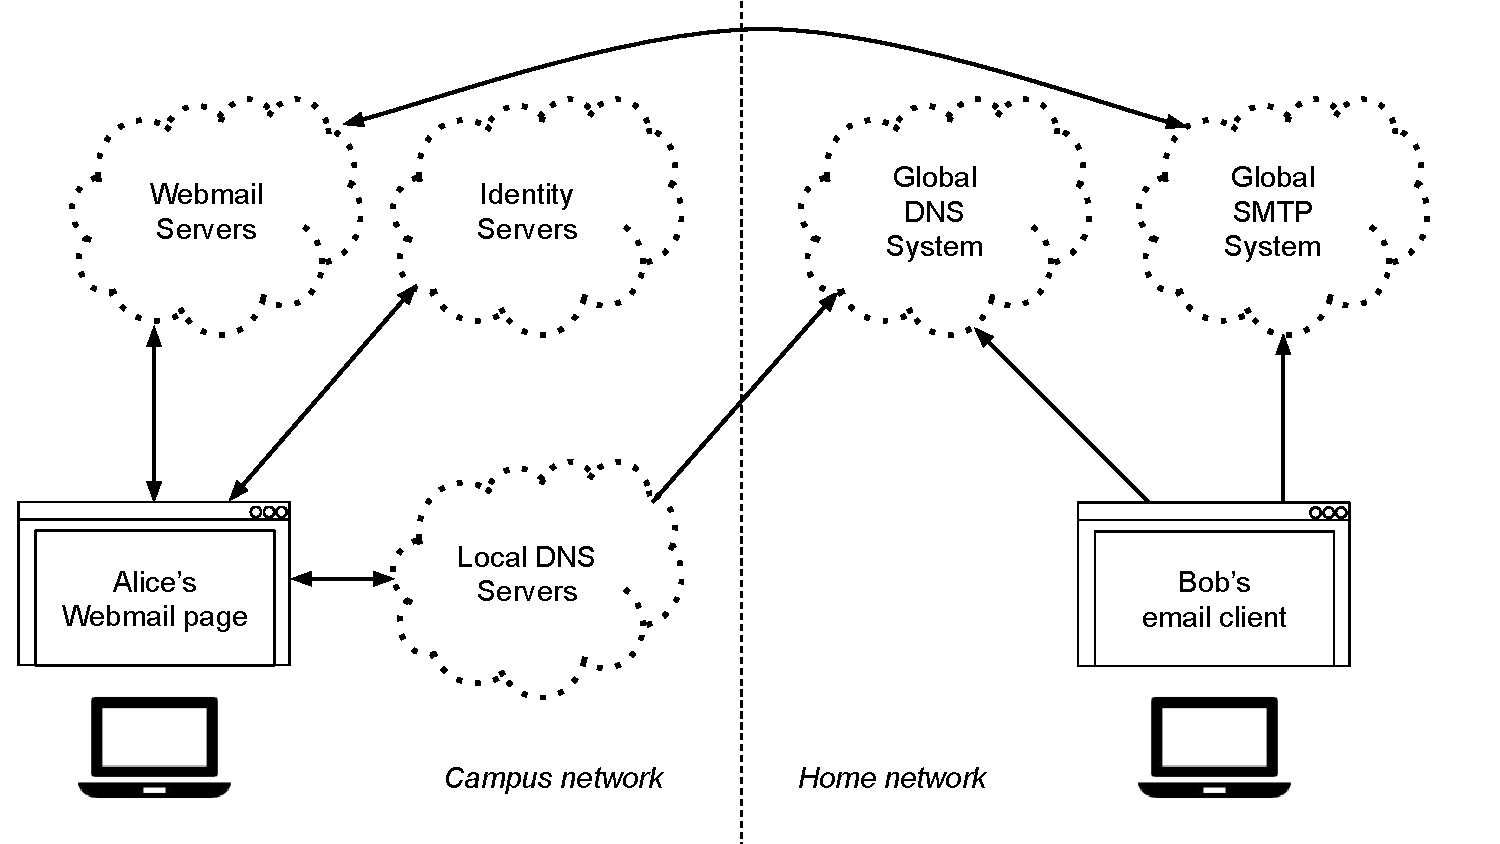
\includegraphics[width=0.9\textwidth,page=1]{figures/dissertation-figures}
   \label{fig:chap1-system-of-systems}
\end{figure}

This thesis is concerned with helping developers build
system-of-systems applications on top of third-party \emph{cloud storage},
\emph{content distribution networks} (CDNs), and \emph{curated data-sets}.
Cloud storage acts as the read/write storage medium for the
application's state.  CDNs help applications overcome high latencies and
bandwidth bottlenecks in WAN settings by serving downstream readers cached data.
Curated datasets host read-only data on behalf of a set of applications, providing value
to each one without requiring them to individually go out and
collect data.

These three types of services are of interest because they implement a
minimal set of requirements for many more applications and services.  For
example, the application and service offerings from Google are
realized with shared corporate cloud storage (i.e. Megastore~\cite{megastore},
Spanner~\cite{spanner}, GFS~\cite{gfs}), a shared corporate
CDN~\cite{google-cdn}, and multiple shared repositories of user behavioral data
that assist in machine-learning tasks like 
spam fighting, page ranking, voice recognition, and so on.  Google's public application
platforms are built with these services as
well~\cite{google-appengine}~\cite{google-cloud}.  The situation is similar for
Amazon AWS and Facebook, which use a common core of cloud storage, CDNs, and
curated datasets to implement both their applications and 
higher-level services (like ad placement and logging).

Most applications are not built on top of bespoke datacenters, CDNs, and curated
datasets, but instead rely on third-party service offerrings.  The developer
leases service capacity in order to build their applications.
For example, a navigation application like OpenStreetMap~\cite{openstreetmap}
would host its users' preferred routes, maps, and historic queries in cloud storage,
use a CDN to cache map data in appropriate geographic regions,
and use public weather data aggregated by NOAA~\cite{noaa} to predict how long a commute may take.
As another example, a movie streaming service like Netflix~\cite{netflix} would
host its users' streaming history in cloud storage, use a CDN to accelerate the
delivery of popular media, and curate the catalog of movies as a shared dataset
for its mobile and Web applications.

% why these three?  can we think of production examples?
% * facebook: datacenters for storage, fbcdn for delivery, social graph for 3rd
% party integration
% * google; datacenters for storage, google CDN for delivery, website index and
% user ad behavior for AI applications

% another example: AI/ML datasets

% TODO: numbers from e.g. Gartner about the growth of the cloud services market?
The growth of these public commodity cloud services and the proliferation of
applications using them demonstrates their promise as system-of-systems
building blocks.  Developers do not have to re-invent existing functionality
each time they build a new application.  Instead, they can
purchase metered service capacity to handle their applications' needs.
This reduces time-to-market, speeds up product iteration, externalizes
infrastructure maintenance and costs,
and lowers the barrier to entry for building new applications.

The difficulty with this approach is that \emph{developers spend lots of
time and effort preserving end-to-end storage semantics}.  This is because an application's
storage semantics depend on the semantics of each cloud service it uses.

To build a correct implementation, developers must account for
the semantics of their chosen services in the application's design.
For example, the aforementioned navigation application's servers
must coordinate with downstream CDN servers to ensure that
clients read fresh data.  As another example, the Web servers in the
campus Webmail application must coordinate with 
the authentication servers to enforce campus-wide access controls.
These concerns are not part of the business logic of the applications, but 
nevertheless must be addressed in order for the application to behave correctly.

\subsection{Challenges}

% government institutions can't use 3rd party clouds (cite conversation)
% is there a law we can cite? a policy doc?
This thesis addresses the challenges of preserving end-to-end storage semantics
in wide-area applications built from third-party cloud services.  Three specific
pain-points are identified.

First, \emph{developers have no control over the services' semantics}.
Cloud services can unilaterally
change their pricing, feature-set, APIs, semantics, availability, and
trustworthiness.  Applications that rely on a service can break unexpectedly
when the service changes its behaviors, and in doing so,
cost developers unforeseeable amounts of time and money.

Developers agree to this one-way relationship when accepting the service's terms of service.  The terms of
service for popular services explicitly state that the operators have the ability to affect unilateral
changes.  For example, Dropbox unilaterally broke its API from version 1 to version
2~\cite{dropbox-v2-api-psa}, and Twitter dropped its API only after non-trivial
applications were built to leverage it~\cite{twitter-api-deprecation-psa}.

The second challenge is that \emph{cloud services are heterogeneous}, which
makes it hard to change both services and end-to-end semantics once the application is deployed.
In practice, services that fill similar roles do not always offer the same semantics.
For example, a service designed to use a single Amazon S3 bucket may 
depend on its sequential consistency, which may prevent the developer from
switching to Microsoft OneDrive (which provides eventual
consistency~\cite{consistency-comparison-cloud-storage}) even though both
services fulfill a cloud storage role.   % https://blog.cloudrail.com/compare-consistency-models-of-cloud-storage-services/

Without careful planning, the application can become coupled
to its services by accidentally relying on undocumented or unacknowledged
behavior.  This creates high service switching costs, making it
difficult for developers to move the application to better
offerrings or change the application's semantics later to meet new requirements.

The third challenge is that \emph{system-of-systems applications
span multiple autonomous organizations}.  An \emph{organization} is an autonomous set of computers that
adhere to a single data-hosting policy for the data their user(s) produce.
Example organizations include a user's personal devices,
a corporation's workstations, or a lab's compute cluster.  Its data-hosting policy
encodes rules like access controls, replica placement, data retention,
and so on that the organization needs enforced on its application data.

Developers need to respect each organization's autonomy.
Each organization needs to be free to
set its own data-hosting policy, and developers need to ensure that its
rules are followed without affecting the end-to-end storage semantics.
This is true of the example Webmail application, since the campus-hosted
servers, the SMTP servers, and the DNS servers can each
decide how they store their message and routing information
without affecting the store-and-forward semantics of email.

The difficulty of building cross-organization applications arises from the
degree to which organizations are willing to trust other organizations to enforce
their policies.  This degree of trust falls on a spectrum.
At one extreme, organizations do not trust other organizations with policy
enforcement on their data.  The designs of applications at this extreme reflect this by requiring
each organization to host their own data, thus putting them in a position to
mediate all accesses to it.
The campus Webmail example falls into this extreme, as do most federated
applications like IRC~\cite{irc}, XMPP~\cite{xmpp},
Diaspora~\cite{diaspora}, and Mastadon~\cite{mastadon}.

At the other extreme,
organizations fully trust external organizations.
The designs of applications at this extreme allow each organization to completely delegate
policy enforcement to another organization.  Examples include most Web services like 
Facebook~\cite{facebook}, Google Apps~\cite{gapps}, and Microsoft
Office 365~\cite{microsoft-apps}, where each organization completely trusts the company running
the application to enforce its data policies.

At both extremes, policy enforcement mechanisms are
straightforward to develop, since the mechanism is deployed within the
organization that also happens to host the data to which the policy
applies.  However, applications built on cloud services
fall in-between these two extremes.  In these applications, the data policy
enforcement mechanisms are \emph{not necessarily} deployed in the same
organization that hosts the data.

In applications build on cloud services, organizations
at a minimum trust the cloud services to keep their data available.
They may also trust them with additional
responsibilities on a case-by-case basis,
such as domain-specific access controls or replica placement.
The policy rules for each application and each organization can be arbitrary.

The challenge to developers is to accommodate the \emph{whole spectrum} of
organizations' trust relationships with cloud services.
Each organization not only has different
policies, but also has different degrees of trust in the services to meet them.
This affects the design of the policy enforcement mechanisms, such that
in the limit, the developers must write a besopke mechanism
for each organization.  This is a much costlier development proposition than the extreme
cases, since not only can the cost to add a new organization require bespoke
code, but also the mechanisms must all be developed in a way that keeps them
interoperable with one another and compatible with the end-to-end storage
semantics.

% DONE
% add a subsection: problem statement (crisp statement)
% make sure chapter 2's objectives tightly link to this problem statement
% distilled design principles: link back to this problem statement
% goal: be able to read 1.1.1, 1.1.2, 2.1, and 2.9, and "get it".
% challenges and objectives are *duals* of each other.
% requirements are derived from objectives, but one layer deeper.
% 2.3-2.8 are the meat.
% 2.9 connects the dots, back to the challenges.
\subsection{Problem Statement}

Building applications on cloud services forces developers to solve two hard
problems in practice.

\begin{itemize}
   \item \textbf{Preserve end-to-end storage semantics}.  This is difficult
      today because developers do not
      control the services' storage semantics.  The services can change their
      behavior, the developers can change the services the application uses, and
      the developers can change the semantics of the application.
      The consequences are the same in all cases:  the developers need to patch the application to
      accommodate the new semantics.

   \item \textbf{Preserve organizational autonomy}.  This is difficult today
      because applications run across multiple organizations,
      and each organization has its own policies about how
      its data should be hosted.  However, neither the developers nor the organizations
      control the services, and organizations have varying degrees of trust in
      each service's ability to accommodate its policies.
      In the limit, this forces developers to come up with
      per-organization policy enforcement mechanisms.
\end{itemize}

As a result, developers spend a lot of time and effort patching their
application just to keep it running.  This thesis shows developers how to
address both problems in a way that requires minimal additional work once the
application is deployed.

\section{Wide-area Software-defined Storage}

% TODO: this is too brief...show examples above?
% TODO: won't applications run the same risks with SDS as they do with cloud
% services?  can we argue that SDS is somehow more stable than these services?

To address these problems, this thesis presents a 
storage architecture that separates storage semantics
from both cloud services and applications.  The rules for processing reads and writes
are placed in a common data-exchange
layer in-between applications and the cloud services.  A system that
implements this layer is called a \emph{wide-area software-defined storage} (SDS) system
(Figure~\ref{fig:chap1-sds-overview}).

\begin{figure}[h]
   \caption{Software-defined storage acts as an intermediate ``narrow waist''
   layer that preserves application-specific storage semantics on top of
   commodity cloud services.}
   \centering
   \includegraphics[width=0.9\textwidth,page=28]{figures/dissertation-figures}
   \label{fig:chap1-sds-overview}
\end{figure}

SDS systems preserve end-to-end storage semantics on top of cloud services while respecting
organizational autonomy.  A SDS system accommodates changes in service semantics
by encapsulating service-specific interfacing logic inside a ``service driver.''
The service driver gives the SDS system a very simple API for loading and
storing immutable chunks of data.  This isolates a particular service from the rest of the
system and makes its functionality accessible via a common API.  Once the SDS system has a
driver implementation for a service, any SDS-powered application can use it
automatically.

SDS preserves organizations' autonomy without compromising end-to-end semantics by
allowing developers to control the network paths the data takes from the application to
the services (and vice versa).  Each organization runs its own
service driver instances for storing its data, and developers
route application requests across organizations by means of an ``aggregation driver.''

The aggregation driver is an SDS-specific programming concept that developers
use to implement end-to-end storage semantics.  Its
programming model borrows from both the UNIX shell programming and software-defined
network programming philosophies.  The developer writes an aggregation driver as a
series of composable ``stages,'' which are evaluated in sequential order by the
SDS system to process an application request according to the desired semantics.
Each organization runs one or more aggregation driver stage instances in order to ensure
that its users' reads and writes are processed according to its data-hosting
policy.

SDS systems avoid the problem of service lock-in by means of a ``gateway''.
Each organization runs their service drivers and aggergation driver stages
within SDS gateways they control, and the SDS system routes reads and writes
through a valid sequence of gateways to preserve end-to-end storage semantics.
Each gateway implements the storage API of the
organization's choice, and serves as the application's access point to the SDS
system.  This allows each organization to choose which APIs are exposed to their
applications, and enables each organization to make its on decisions on how its
applications interact with its data.

\begin{figure}[h]
   \caption{Overview of the relationship between service drivers, aggregation
   drivers, and gateways on a read request.  The application's request ``read \texttt{foo}'' is
   processed by a sequence of three aggregation driver stages before
   \texttt{foo}'s data is returned.  The SDS system ensures that each stage is
   executed in the right sequence (preserving semantics),
   and each organization runs a service driver to loads and stores the
   necessary data to do so (preserving autonomy).}
   \centering
   \includegraphics[width=0.9\textwidth,page=33]{figures/dissertation-figures}
   \label{fig:chap1-sds-implementation-overview}
\end{figure}

The resulting system solves both problems
(Figure~\ref{fig:chap1-sds-implementation-overview}).
It ensures that all reads and writes pass through the
correct sequence of aggregation driver
stages, thereby preserving the end-to-end semantics.  At the same time, developers 
control which organizations' aggregation driver stages and service driver
instances are utilized to process a given request.  This lets the organization
enforce their data policies on each request without violating end-to-end
storage semantics.  A detailed description of how service drivers, aggregation
drivers, and gateways coordinate to achieve this is presented in
Chapter~\ref{chap:design_principles}.

\section{Contributions}

The architecture put forth in this thesis is informed by two real-world SDS
implementations and three sample applications.  The implementations were 
designed to accommodate two sets of real-world use-cases: scientific computing,
and ``serverless'' Web applications (i.e. Web applications that can operate
without application-specific servers).
The design principles in this thesis 
were formulated once the implementations were tested and
deployed in production settings.  This thesis claims the following contributions:

\begin{itemize}

\item This thesis presents the design principles of wide-area software-defined storage, framed in
terms of prior work and the real-world storage needs of existing applications.
Adhering to these design principles reduces the man-hours required to keep applications compatible
with existing services while both preserving end-to-end storage semantics and
respecting each organization's data-hosting policies (Chatper~\ref{chap:design_principles}).

\item This thesis presents the design and implementation of two SDS systems: Gaia and
Syndicate.  Syndicate is a real SDS system being deployed in scientific
workflows today, and Gaia is a real SDS system being deployed to build
serverless Web applications.
This thesis uses Gaia and Syndicate to show how to translate SDS design
principles into real systems.
(Chapter~\ref{chap:syndicate_sds}).

\item This thesis shows how to build SDS-powered applications.  The design and
implementation of non-trivial SDS-powered applications \emph{that could not
have been feasibly built without SDS} are presented.  Among these are an end-to-end encrypted
Webmail client that removes the user from key management, a server-less
groupware application that lets users control how their data gets hosted and
accessed, and a scientific data-staging application that
automatically makes fresh datasets available from existing data repositories to
HPC clusters via commodity CDNs.
(Chapter~\ref{chap:applications}).

\item This thesis presents microbenchmarks for Gaia and Syndicate.  The
microbenchmarks show the various overheads of these SDS implementations when
compared to reading and writing data directly to cloud services (i.e. with no
concern for semantics or organizational autonomy).  The results show that the SDS
system imposes modest overhead, and only when enforcing certain safety
properties (Chapter~\ref{chap:evaluation}).

\end{itemize}

These contributions support the thesis that developers can both preserve
end-to-end storage semantics and respect organizational autonomy when building
on cloud services.  A properly-designed SDS system achieves this by framing the
problem in terms of service drivers and aggregation drivers, which can be
written once and reused across applications.  In doing so, SDS systems minimize the amount of
work required to keep an application running.

% TODO: reinforce/tie back to end-to-end storage semantics
% "these four contributions support the thesis that a properly-designed SDS
% system preserves end-to-end semantics..."


